\documentclass[11pt]{article}

\usepackage[colorlinks,urlcolor=blue,linkcolor=blue]{hyperref}
\usepackage{graphicx}
\usepackage[footnotesize]{subfigure}
\usepackage{listings}

 \topmargin 0.in  \headheight 0pt  \headsep 0pt  \raggedbottom
 \oddsidemargin 0.1in 
 \textheight 9.25in  \textwidth 6.00in 
 \parskip 5pt plus 1pt minus 1pt
 \def \baselinestretch {1.25}   % one-and-a-half spaced
 \setlength {\unitlength} {0.75in}
%
%
\newenvironment{routine}[2]
{\vspace{.25in}{\noindent\bf\hspace{0pt} #1}{\\ \noindent #2}
\begin{list}{}{
\renewcommand{\makelabel}[1]{{\tt ##1} \hfil} 
\itemsep 0pt plus 1pt minus 1pt
\leftmargin  1.2in
\rightmargin 0.0in
\labelwidth  1.1in
\itemindent  0.0in
\listparindent  0.0in
\labelsep    0.05in}
}{\end{list}}
%

\begin{document}

\title{OP2 Airfoil Example}
\author{Mike Giles, Gihan Mudalige, Istv{\'a}n Reguly}
\maketitle

\newpage




\tableofcontents

\newpage


\newpage
\section{Introduction}

Airfoil, is an industrial representative CFD application benchmark, written using OP2's C/C++ API. In this document we
detail its development using OP2 and is a guide to application developers wishing to write applications using the OP2
API and framework. 

\noindent Full details of OP2 can be found at: \url{http://www.oerc.ox.ac.uk/research/op2}

Airfoil is a non-linear 2D inviscid airfoil code that uses an unstructured grid. It is a finite volume application that
solves the 2D Euler equations using a scalar numerical dissipation. The algorithm iterates towards the steady state
solution, in each iteration using a control volume approach - for example the rate at which the mass changes within a
control volume is equal to the net flux of mass into the control volume across the four faces around the cell. This is
representative of the 3D viscous flow calculations OP2 supports for production-grade CFD applications (such as the
Hydra~\cite{11,12} CFD code at Rolls Royce plc.). The Airfoil code consists of five parallel loops: \texttt{save\_soln},
\texttt{adt\_calc}, \texttt{res\_calc}, \texttt{bres\_calc} and \texttt{update}. Out of these, \texttt{save\_soln} and
\texttt{update} are direct loops while the other three are indirect loops. The standard mesh size solved with Airfoil
consists of 1.5M edges. In such a mesh the most compute intensive loop, \texttt{res\_calc}, is called 2000 times during
the total execution of the application and performs about 100 floating-point operations per mesh edge. Extensive
performance analysis of Airfoil and optimisations have been detailed in our published work~\cite{PER2011, CJ2011,
PER2012, InPar2012}. What follows is a step-by-step treatment of the stages involved in developing Airfoil. The
application and generated code can be found under \texttt{OP2-Common/apps/c/airfoil}.\vspace{-5pt}

\section{Airfoil - The Development CPU Version}

For the application developer wishing to utilise the OP2 framework for developing unstructured mesh codes, the first
step is to develop the application assuming that the target execution system is a traditional single threaded CPU.
This simplifies the programming complexity of the code by allowing the developer to concentrate on the application
domain and science involved and not the intricacies of parallel programming. During development the code can be run
without any OP2 code generation, on a single CPU thread by simply including the \texttt{op\_seq.h} header file. 

The Airfoil application level code (i.e. the code written by the domain scientist) consists of only a main function (in
\texttt{airfoil.cpp}) where it performs a time marching loop that executes 1000 times, each time calling the above
mentioned five loops. Each loop iterates over a specified \texttt{op\_set} and the operations to be performed per
iteration are detailed in a header file for each loop: \texttt{save\_soln.h, adt\_calc.h, res\_calc.h, bres\_calc.h} and
\texttt{update.h}. The following code illustrates the declaration of the \texttt{res\_calc} loop, which iterates over
the edges of the mesh.


\begin{figure}\small
\vspace{-0pt}\noindent\line(1,0){8}\vspace{-10pt}
\begin{lstlisting}
//  calculate flux residual
    op_par_loop(res_calc,"res_calc",edges,
          op_arg_dat(p_x,    0,pedge, 2,"double",OP_READ),
          op_arg_dat(p_x,    1,pedge, 2,"double",OP_READ),
          op_arg_dat(p_q,    0,pecell,4,"double",OP_READ),
          op_arg_dat(p_q,    1,pecell,4,"double",OP_READ),
          op_arg_dat(p_adt,  0,pecell,1,"double",OP_READ),
          op_arg_dat(p_adt,  1,pecell,1,"double",OP_READ),
          op_arg_dat(p_res,  0,pecell,4,"double",OP_INC ),
          op_arg_dat(p_res,  1,pecell,4,"double",OP_INC ));
\end{lstlisting}\vspace{-10pt}
\vspace{-0pt}\noindent\line(1,0){8}\vspace{-10pt}
\caption{\small res\_calc loop}
\normalsize\vspace{-10pt}\label{fig:rescalc}
\end{figure}

\noindent The first argument specifies the name of the function (implemented in \texttt{res\_calc.h}) that contains the
operations to be performed per iteration in the loop. The second argument notes the name of the loop, while the third
specifies the \texttt{op\_set} over which the loop will iterate. The remaining arguments specify the access descriptors
of the data used in the loop. More details of the \texttt{op\_arg\_dat} API statements are given in the user guide.

For Airfoil, \texttt{airfoil.cpp} include the OP2 header files and the elemental kernel header files as follows.
Additionally global constants must be declared before the \texttt{main()} function.

\begin{figure}[!h]\small
\vspace{-0pt}\noindent\line(1,0){8}\vspace{-10pt}
\begin{lstlisting}
// OP2 header file
#include "op_seq.h"

// global constants
double gam, gm1, cfl, eps, mach, alpha, qinf[4];

// user kernel routines for parallel loops
#include "save_soln.h"
#include "adt_calc.h"
#include "res_calc.h"
#include "bres_calc.h"
#include "update.h"
\end{lstlisting}\vspace{-10pt}
\vspace{-0pt}\noindent\line(1,0){8}\vspace{-10pt}
\caption{\small Header and global constants }
\normalsize\vspace{-10pt}\label{fig:header}
\end{figure}

\noindent The main function of an OP2 applications need to begin with the initialisation statement \texttt{op\_init()}
before any other OP2 API statements can be called. The Airfoil application then reads in the input mesh file. As
detailed in the user documentation, OP2 allows the application developer to carry out their own I/O or utilise hdf5
based I/O using OP2's hdf5 API statements. We first detail the development of Airfoil assuming that file I/O is
implemented by the application developer. Later in Section~\ref{hdf5} we will detail the Airfoil application written
utilising OP2's hdf5 file I/O capabilities. 

Assume that the application reads an ASCI file using standard C++ file I/O statements to read in the input mesh and
allocate memory to hold the data. The data is then passed to the appropriate OP2 declaration statements to declare
\texttt{op\_set}s, \texttt{op\_map}s and \texttt{op\_dat}s as follows:

\begin{figure}[!h]\small
\vspace{-0pt}\noindent\line(1,0){8}\vspace{-10pt}
\begin{lstlisting}
  op_set nodes  = op_decl_set(nnode,  "nodes");
  op_set edges  = op_decl_set(nedge,  "edges");
  op_set bedges = op_decl_set(nbedge, "bedges");
  op_set cells  = op_decl_set(ncell,  "cells");

  op_map pedge   = op_decl_map(edges, nodes,2,edge,  "pedge");
  op_map pecell  = op_decl_map(edges, cells,2,ecell, "pecell");
  op_map pbedge  = op_decl_map(bedges,nodes,2,bedge, "pbedge");
  op_map pbecell = op_decl_map(bedges,cells,1,becell,"pbecell");
  op_map pcell   = op_decl_map(cells, nodes,4,cell,  "pcell");

  op_dat p_bound = op_decl_dat(bedges,1,"int"   , bound ,"p_bound");
  op_dat p_x     = op_decl_dat(nodes ,2,"double", x     ,"p_x");
  op_dat p_q     = op_decl_dat(cells ,4,"double", q     ,"p_q");
  op_dat p_qold  = op_decl_dat(cells ,4,"double", qold  ,"p_qold");
  op_dat p_adt   = op_decl_dat(cells ,1,"double", adt   ,"p_adt");
  op_dat p_res   = op_decl_dat(cells ,4,"double", res   ,"p_res");

  op_decl_const(1,"double",&gam  );
  op_decl_const(1,"double",&gm1  );
  op_decl_const(1,"double",&cfl  );
  op_decl_const(1,"double",&eps  );
  op_decl_const(1,"double",&mach );
  op_decl_const(1,"double",&alpha);
  op_decl_const(4,"double",qinf  );
\end{lstlisting}\vspace{-10pt}
\vspace{-0pt}\noindent\line(1,0){8}\vspace{-10pt}
\caption{\small OP2 set, map and dat declarations }
\normalsize\vspace{-10pt}\label{fig:decls}
\end{figure}

\noindent Four sets are declared (\texttt{nodes, edges, bedges} and \texttt{cells}) and five mappings between sets are
declared to establish connectivity between sets. The six data arrays are declared on the sets \texttt{bedges, nodes} and
\texttt{cells}. Any constants used by the program are also declared at this point using \texttt{op\_decl\_const()}.
The five parallel loops that make up the Airfoil application are detailed next within a time-marching loop.
\begin{figure}[!h]\small
\vspace{-0pt}\noindent\line(1,0){8}\vspace{-10pt}
\begin{lstlisting}
//main time-marching loop
for(int iter=1; iter<=niter; iter++) {
    // save old flow solution
    op_par_loop(save_soln, ... );

    // predictor/corrector update loop
    for(int k=0; k<2; k++) {

      // calculate area/timstep
      op_par_loop(adt_calc, ... );

      // calculate flux residual
      op_par_loop(res_calc, ... );

      op_par_loop(bres_calc, ... );
      
      // update flow field
      op_par_loop(update, ... );
    }
    ...
}
\end{lstlisting}\vspace{-10pt}
\vspace{-0pt}\noindent\line(1,0){8}\vspace{-10pt}
\caption{\small Time marching loop }
\normalsize\vspace{-10pt}\label{fig:timemarching}
\end{figure}

Finally, statistics about the performance of the application can be printed to stdout using
\texttt{op\_timing\_output()} and OP2 is terminated with \texttt{op\_exit()}, deallocating internal OP2 allocated
memory. If the application developer allocated memory, for example to read in the mesh, then he/she will need to
manually deallocate memory at this point. 

During development, by simply including the \texttt{op\_seq.h} header file application can be compiled by a conventional
compiler (gcc, icc etc.) to produce an executable that can be run on a single threaded CPU. No code generation is
required at this stage, where the application developer is only using the single threaded executable for debugging and
development. This enable the developer to build the application and test its accuracy without considering any
parallelisation issues. The compilation of the application for single-threaded CPUs is achieved by linking with the OP2
sequential library \texttt{libop2\_seq.a}, for example as follows:

\begin{figure}[!h]\small
\vspace{-0pt}\noindent\line(1,0){8}\vspace{-10pt}
\begin{lstlisting}
OP2_INC         = -I$(OP2_INSTALL_PATH)/c/include
OP2_LIB         = -L$(OP2_INSTALL_PATH)/c/lib
CPP             = icpc
CPPFLAGS         = -O3 -xSSE4.2 
airfoil_seq: airfoil.cpp save_soln.h adt_calc.h res_calc.h \
	      bres_calc.h update.h
             $(CPP) $(CPPFLAGS) airfoil.cpp \
             $(OP2_INC) $(OP2_LIB) -lop2_seq -o airfoil_seq 
\end{lstlisting}\vspace{-10pt}
\vspace{-0pt}\noindent\line(1,0){8}\vspace{-10pt}
\caption{\small Sequential developer version build }
\normalsize\vspace{-10pt}\label{fig:seqbuild}
\end{figure}

\noindent Once the application is debugged and tested on a single CPU, OP2's code generation capabilities can be used
to generate executables for different parallel architectures. We will use OP2's Python code parser for code generation
throughout this document. The various back-ends supported by OP2, and their build process are detailed in
Figure~\ref{fig/build-paths}. 

\begin{figure}[!ht]\centering\vspace{0pt}
\subfigure[Single-Node build]{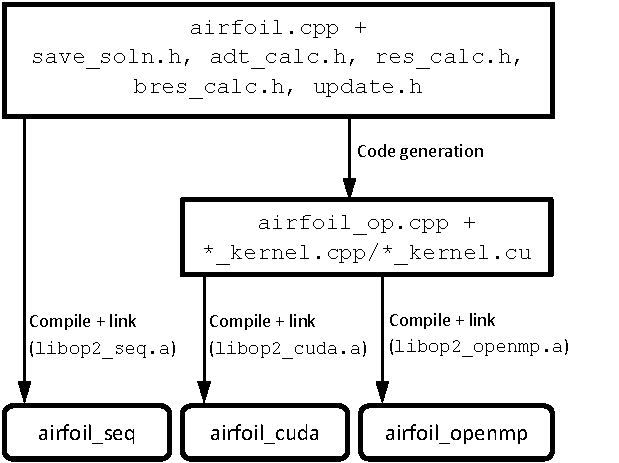
\includegraphics[width=9cm]{airfoil_plain}\vspace{-0pt}}
\subfigure[MPI Build]{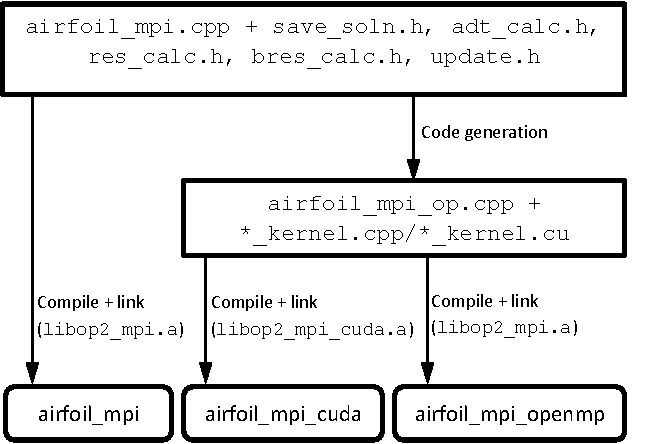
\includegraphics[width=9cm]{airfoil_plain_mpi}\vspace{-0pt}}
\caption{Code generation and build for Airfoil (with user I/O)}\label{fig/build-paths}\vspace{-5pt}
\end{figure}

\noindent Figure~\ref{fig/build-paths} assumes that the user is responsible for performing the required I/O for the
application. As such \texttt{airfoil\_mpi.cpp} will be an MPI application written by the user utilising his/her own
parallel I/O as will be detailed in Section~\ref{sec/mpi}. As mentioned before, the single CPU Airfoil application
(\texttt{airfoi\_seq}) can be built without any code generation. Similarly the distributed memory MPI application,
\texttt{airfoi\_mpi}, for executing on a single threaded cluster of CPUs, also can be built without code generation
(see Section ~\ref{sec/mpi}). The current OP2 code generation tools can be applied to the above two versions of the
application to generate code for parallel execution on (1) a single GPU using NVIDIA CUDA, (2) Multi-threaded CPU using
OpenMP, (3) cluster of GPUs using MPI+CUDA and (4) a cluster of multi-threaded CPUs using MPI+OpenMP. In order to obtain
the code for these targets, the code generator will need to be applied \underline{\textbf{two times}}, once to
\texttt{airfoil.cpp} and then to \texttt{airfoil\_mpi.cpp}. The former will generate a modified main program and
kernel files for single node parallel execution and the latter will generate code for parallel execution on a
heterogeneous distributed memory cluster. 

\noindent The code generator needs to be invoked, for example for parsing \texttt{airfoil.cpp}:

$\$>$ ./op2.py airfoil.cpp

\noindent For parsing \texttt{airfoil\_mpi.cpp}, to generate the distributed memory code:

$\$>$ ./op2.py airfoil\_mpi.cpp

\noindent More specific details of the build process for each target back-end is detailed in the next sections. 

\newpage
\section{Generating Single Node OpenMP and CUDA Executables}\label{sec/cuda_openmp}
This section will detail generating code for a single CPU node (SMP or CMP node) or a single GPU, using OpenMP and
NVIDIA CUDA respectively. 

The code generator will produce a modified main program and back-end specific code. In this case \texttt{airfoil.cpp}
will be transformed to \texttt{airfoil\_op.cpp} and a kernel file will be produced corresponding to each
\texttt{op\_par\_loop} in the main program (\texttt{*\_kernel.cpp} for OpenMP and \texttt{*\_kernel.cu} for CUDA). For
running on SMP CPU nodes, OpenMP is utilised. The executable can be built by compiling the code with a conventional C++
compiler and linking with the openmp back-end library, \texttt{libop2\_openmp.a}, for example as follows:

\begin{figure}[!h]\small
\vspace{-0pt}\noindent\line(1,0){8}\vspace{-10pt}
\begin{lstlisting}
OP2_INC         = -I$(OP2_INSTALL_PATH)/c/include
OP2_LIB         = -L$(OP2_INSTALL_PATH)/c/lib
CPP             = icpc
CPPFLAGS        = -O3 -xSSE4.2 
OMPFLAGS        = -openmp -openmp-report2
airfoil_openmp:	airfoil_op.cpp airfoil_kernels.cpp \
                save_soln_kernel.cpp save_soln.h \
                adt_calc_kernel.cpp adt_calc.h \
                res_calc_kernel.cpp res_calc.h \
                bres_calc_kernel.cpp bres_calc.h \
                update_kernel.cpp update.h \
                $(CPP) $(CPPFLAGS) $(OMPFLAGS) $(OP2_INC) $(OP2_LIB) \
                airfoil_op.cpp airfoil_kernels.cpp \
                -lm -lop2_openmp -o airfoil_openmp
\end{lstlisting}\vspace{-10pt}
\vspace{-0pt}\noindent\line(1,0){8}\vspace{-10pt}
\caption{\small OpenMP version build }
\normalsize\vspace{-10pt}\label{fig:ompbuild}
\end{figure}


\noindent The \texttt{airfoil\_kernels.cpp} includes all the \texttt{*\_kernel.cpp} files. This is why it is the only
file appearing in the compile line. The \texttt{airfoil\_openmp} can be run on multiple OpenMP threads by setting the
\texttt{OMP\_NUM\_THREADS} environmental variable.\newpage

\noindent For running on a single GPU, NVIDIA CUDA is utilised. The executable can be built by compiling with nvcc and a
conventional C++ compiler and linking with the CUDA back-end library, \texttt{libop2\_cuda.a}, for example as follows:

\begin{figure}[!h]\small
\vspace{-0pt}\noindent\line(1,0){8}\vspace{-10pt}
\begin{lstlisting}
OP2_INC         = -I$(OP2_INSTALL_PATH)/c/include
OP2_LIB         = -L$(OP2_INSTALL_PATH)/c/lib
CPP             = icpc
CPPFLAGS         = -O3 -xSSE4.2 
CUDA_INC        = -I$(CUDA_INSTALL_PATH)/include
CUDA_LIB        = -L$(CUDA_INSTALL_PATH)/lib64
NVCCFLAGS       = -O3 -arch=sm_20 -Xptxas=-v -Dlcm=ca -use_fast_math 
airfoil_cuda:	airfoil_op.cpp airfoil_kernels_cu.o
                $(CPP) $(CPPFLAGS) $(CUDA_INC) $(OP2_INC) \
                $(OP2_LIB) $(CUDA_LIB) \
                airfoil_op.cpp airfoil_kernels_cu.o -lcudart \
               -lop2_cuda -o airfoil_cuda                                      

airfoil_kernels_cu.o:	airfoil_kernels.cu      \
                save_soln_kernel.cu save_soln.h \
                adt_calc_kernel.cu  adt_calc.h  \
                res_calc_kernel.cu  res_calc.h  \
                bres_calc_kernel.cu bres_calc.h \
                update_kernel.cu    update.h    \
                nvcc $(NVCCFLAGS) $(OP2_INC) \
                -c -o airfoil_kernels_cu.o \
                airfoil_kernels.cu
\end{lstlisting}\vspace{-10pt}
\vspace{-0pt}\noindent\line(1,0){8}\vspace{-10pt}
\caption{\small CUDA version build }
\normalsize\vspace{-10pt}\label{fig:cudabuild}
\end{figure}

\noindent Similar to the OpenMP compilation, the \texttt{airfoil\_kernels.cu} includes all the \texttt{*\_kernel.cu}
files. When \texttt{airfoil\_cuda} is executed, it will select any available GPU  on the system. The GPU to be selected
can be set by using the \texttt{CUDA\_VISIBLE\_DEVICES} environment variable. 

\newpage
\section{Building Airfoil for Distributed Memory (MPI) Execution}\label{sec/mpi}

If the application developer decides to be responsible for the application's I/O, i.e. for reading in the unstructured
mesh, then for distributed memory execution of the application, parallelising the I/O process cannot be simply
automated. As such OP2's code generation tools does not support generating an MPI based application, by simply parsing
\texttt{airfoil.cpp}. What is required is the development of \texttt{airfoil\_mpi.cpp} that explicitly codes the
parallel I/O. The only difference between \texttt{airfoil.cpp} and \texttt{airfoi\_mpi.cpp} is that the latter hands
partitions of the \texttt{op\_set}s, \texttt{op\_map}s and \texttt{op\_dat}s that resides on each MPI process to OP2 via
\texttt{op\_decl\_*} statements (see \texttt{OP2-Common/airfoil/dp/airfoi\_mpi.cpp}). OP2 supports the coding of such an
MPI application, without the need for any code generation. Similar to the development process for a single threaded CPU,
all that is required is to include the \texttt{op\_seq.h} header file. The MPI application can be built by compiling
with mpiCC and linking with the MPI back-end library, \texttt{libop2\_mpi.a}, for example as follows:

\begin{figure}[!h]\small
\vspace{-0pt}\noindent\line(1,0){8}\vspace{-10pt}
\begin{lstlisting}
MPICPP          = mpiCC
MPIFLAGS        = -O3 -xSSE4.2 

PARMETIS_INC    = -I$(PARMETIS_INSTALL_PATH) -DHAVE_PARMETIS
PARMETIS_LIB    = -L$(PARMETIS_INSTALL_PATH) -lparmetis \
                  -L$(PARMETIS_INSTALL_PATH) -lmetis

PTSCOTCH_INC    = -I$(PTSCOTCH_INSTALL_PATH)/include -DHAVE_PTSCOTCH
PTSCOTCH_LIB    = -L$(PTSCOTCH_INSTALL_PATH)/lib/ -lptscotch \
                  -L$(PTSCOTCH_INSTALL_PATH)/lib/ -lptscotcherr

airfoil_mpi: airfoil_mpi.cpp \
        save_soln.h adt_calc.h res_calc.h bres_calc.h Makefile
        $(MPICPP) $(MPIFLAGS) $(OP2_INC) \
        $(PARMETIS_INC) $(PTSCOTCH_INC) \
        $(OP2_LIB) airfoil_mpi.cpp -lop2_mpi \
        $(PARMETIS_LIB) $(PTSCOTCH_LIB) -o airfoil_mpi
\end{lstlisting}\vspace{-10pt}
\vspace{-0pt}\noindent\line(1,0){8}\vspace{-10pt}
\caption{\small MPI version build }
\normalsize\vspace{-10pt}\label{fig:mpibuild}
\end{figure}

\noindent The unstructured mesh, will be repartitioned by OP2, using parallel graph/mesh partitioning libraries
(ParMetis or PTScotch) as detailed in the user documentation. Thus linking with the appropriate mesh partitioning
library will also be needed as detailed above. The resulting executable, \texttt{airfoil\_mpi}, can be executed on a
cluster of single threaded CPUs, with the use of the usual mpirun command. 

\newpage
% \section{Heterogeneous Systems}\label{sec/heterogeneous}

Once developed, \texttt{airfoi\_mpi.cpp} can be used to generate the code required to build the application for
execution on distributed memory heterogeneous systems. Currently supported systems, are a cluster of multi-threaded CPUs
(Using MPI and OpenMP) and a cluster of GPUs (using MPI and CUDA).

Similar to the single-node parallel version, the code generator will produce a modified main program and back-end
specific code. In this case \texttt{airfoil\_mpi.cpp} will be transformed to \texttt{airfoil\_mpi\_op.cpp} and a kernel
file will be produced corresponding to each \texttt{op\_par\_loop} in the main program (\texttt{*\_kernel.cpp} for
OpenMP and \texttt{*\_kernel.cu} for CUDA). By design these kernel files will be identical to the kernel files created
for the single-node parallel back-ends. 

\noindent The executable for a cluster of multi-threaded CPUs can be built by compiling the code using a conventional
C++ compiler and linking with the back-end library, \texttt{libop2\_mpi.a}, for example as follows:

\begin{figure}[!h]\small
\vspace{-0pt}\noindent\line(1,0){8}\vspace{-10pt}
\begin{lstlisting}
airfoil_mpi_openmp: airfoil_mpi_op.cpp airfoil_kernels.cpp \
                    save_soln_kernel.cpp  save_soln.h \
                    adt_calc_kernel.cpp   adt_calc.h  \
                    res_calc_kernel.cpp   res_calc.h  \
                    bres_calc_kernel.cpp  bres_calc.h \
                    update_kernel.cpp     update.h    \
                    Makefile
                    $(MPICPP) $(MPIFLAGS) $(OMPFLAGS) \
                    airfoil_mpi_op.cpp \
                    airfoil_kernels.cpp \
                    $(OP2_INC) $(PARMETIS_INC) $(PTSCOTCH_INC) \
                    $(OP2_LIB) -lop2_mpi \
                    $(PARMETIS_LIB) $(PTSCOTCH_LIB) -o airfoil_mpi_openmp
\end{lstlisting}\vspace{-10pt}
\vspace{-0pt}\noindent\line(1,0){8}\vspace{-10pt}
\caption{\small MPI+OpenMP version build }
\normalsize\vspace{-10pt}\label{fig:mpi_openmpbuild}
\end{figure}

\noindent \texttt{airfoil\_mpi\_openmp} needs to be executed using mpirun and will utilise OMP\_NUM\_THREADS per MPI
process on the multi-threaded CPU cluster during execution. 

\newpage
\noindent The executable for a cluster of GPUs can be built by compiling the code using a conventional C++ compiler,
CUDA compiler nvcc and linking with the back-end library, \texttt{libop2\_mpi\_cuda.a}, for example as follows:

\begin{figure}[h]\small
\vspace{-0pt}\noindent\line(1,0){8}\vspace{-10pt}
\begin{lstlisting}
airfoil_mpi_cuda: airfoil_mpi_op.cpp airfoil_kernels_mpi_cu.o Makefile
                  $(MPICPP) $(MPIFLAGS) airfoil_mpi_op.cpp \
                  airfoil_kernels_mpi_cu.o \
                  $(OP2_INC) $(PARMETIS_INC) $(PTSCOTCH_INC) \
                  $(OP2_LIB) -lop2_mpi_cuda $(PARMETIS_LIB) \
                  $(PTSCOTCH_LIB) \
                  $(CUDA_LIB) -lcudart -o airfoil_mpi_cuda

airfoil_kernels_mpi_cu.o:       airfoil_kernels.cu      \
                  save_soln_kernel.cu  save_soln.h \
                  adt_calc_kernel.cu   adt_calc.h  \
                  res_calc_kernel.cu   res_calc.h  \
                  bres_calc_kernel.cu  bres_calc.h \
                  update_kernel.cu     update.h    \
                  Makefile
                  nvcc  $(INC) $(NVCCFLAGS) $(OP2_INC) \
                  -I $(MPI_INSTALL_PATH)/include \
                  -c -o airfoil_kernels_mpi_cu.o airfoil_kernels.cu
\end{lstlisting}\vspace{-10pt}
\vspace{-0pt}\noindent\line(1,0){8}\vspace{-10pt}
\caption{\small MPI+CUDA version build }
\normalsize\vspace{-10pt}\label{fig:mpi_cudabuild}
\end{figure}

\noindent \texttt{airfoil\_mpi\_cuda} needs to be executed using mpirun and will utilise one GPU per MPI process on the
GPU cluster during execution. 

\newpage
\section{Airfoil with HDF5 I/O}\label{hdf5}
If OP2's file I/O is utilised when developing the application then all code required for \underline{\textbf{all}} the
target back-ends will be generated by parsing the \texttt{airfoil.cpp} file. This includes the distributed memory (MPI)
back-ends. The code generation and application build process is summarised in Figure~\ref{fig/build-paths-hdf5}. The
code generator produces a common modified main program in \texttt{airfoil\_op.cpp} and kernel files, which is then
linked with the appropriate OP2 back-ends libraries to give the desired target executable. 

\begin{figure}[ht]\centering\vspace{0pt}
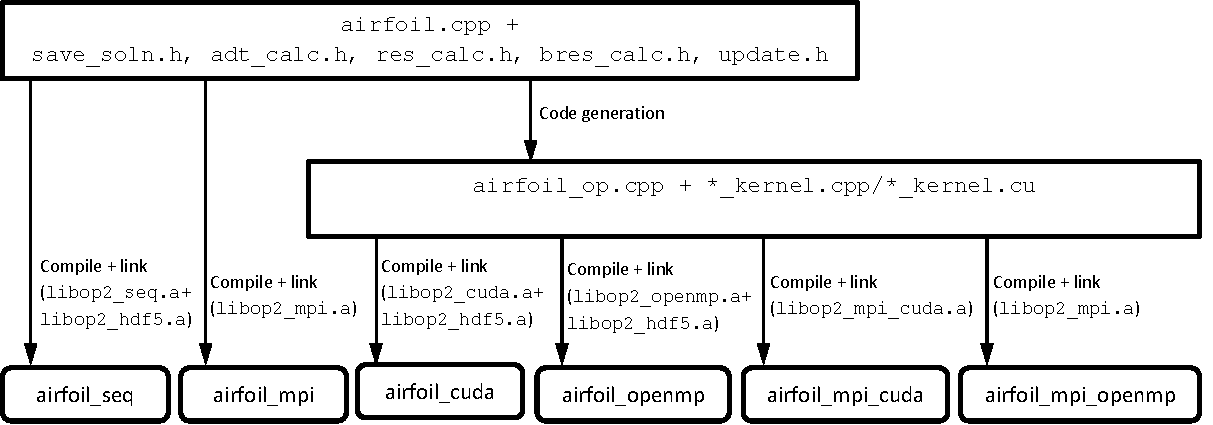
\includegraphics[width=15.5cm]{airfoil_hdf5}\vspace{-0pt}
\caption{Code generation and build for Airfoil (with OP2 HDF5 file I/O)}\label{fig/build-paths-hdf5}\vspace{-5pt}
\end{figure}

\newpage
\noindent The library \texttt{libop2\_hdf5.a} needs to be linked when building single node executables, for example:

\begin{figure}[!h]\small
\vspace{-0pt}\noindent\line(1,0){8}\vspace{-10pt}
\begin{lstlisting}
HDF5_INC = -I$(HDF5_INSTALL_PATH)/include
HDF5_LIB = -L$(HDF5_INSTALL_PATH)/lib -lhdf5 -lz

airfoil_cuda:   airfoil_op.cpp airfoil_kernels_cu.o Makefile
                $(MPICPP) $(CPPFLAGS) airfoil_op.cpp airfoil_kernels_cu.o \
                $(CUDA_INC) $(OP2_INC) $(HDF5_INC) \
                $(OP2_LIB) $(CUDA_LIB) -lcudart -lop2_cuda -lop2_hdf5 \
                $(HDF5_LIB) -o airfoil_cuda

airfoil_kernels_cu.o:   airfoil_kernels.cu      \
                save_soln_kernel.cu save_soln.h \
                adt_calc_kernel.cu  adt_calc.h  \
                res_calc_kernel.cu  res_calc.h  \
                bres_calc_kernel.cu bres_calc.h \
                update_kernel.cu    update.h    \
                Makefile
                nvcc $(INC) $(NVCCFLAGS) $(OP2_INC) $(HDF5_INC) \
                -I /home/gihan/openmpi-intel/include \
                -c -o airfoil_kernels_cu.o airfoil_kernels.cu
\end{lstlisting}\vspace{-10pt}
\vspace{-0pt}\noindent\line(1,0){8}\vspace{-10pt}
\caption{\small CUDA with HDF5 build }
\normalsize\vspace{-10pt}\label{fig:hdf5build}
\end{figure}

\newpage
\noindent On the other hand the functions facilitating MPI parallel file I/O with hdf5 are contained in the MPI back-end
implicitly. Thus linking should not be done with \texttt{libop2\_hdf5.a} in this case, for example:

\begin{figure}\small
\vspace{-0pt}\noindent\line(1,0){8}\vspace{-10pt}
\begin{lstlisting}
HDF5_INC = -I$(HDF5_INSTALL_PATH)/include
HDF5_LIB = -L$(HDF5_INSTALL_PATH)/lib -lhdf5 -lz

airfoil_mpi_cuda: airfoil_op.cpp airfoil_kernels_mpi_cu.o Makefile
                  $(MPICPP) $(MPIFLAGS) airfoil_op.cpp \
                  -lm airfoil_kernels_mpi_cu.o \
                  $(OP2_INC) $(PARMETIS_INC) $(PTSCOTCH_INC) $(HDF5_INC) \
                  $(OP2_LIB) -lop2_mpi_cuda \
                  $(PARMETIS_LIB) $(PTSCOTCH_LIB) \
                  $(HDF5_LIB) $(CUDA_LIB) -lcudart -o airfoil_mpi_cuda
                  
airfoil_kernels_mpi_cu.o: airfoil_kernels.cu \
                save_soln_kernel.cu  save_soln.h \
                adt_calc_kernel.cu   adt_calc.h  \
                res_calc_kernel.cu   res_calc.h  \
                bres_calc_kernel.cu  bres_calc.h \
                update_kernel.cu     update.h    \
                Makefile
                nvcc  $(INC) $(NVCCFLAGS) $(OP2_INC) \
                -I $(MPI_INSTALL_PATH)/include \
                -c -o airfoil_kernels_mpi_cu.o airfoil_kernels.cu
\end{lstlisting}\vspace{-10pt}
\vspace{-0pt}\noindent\line(1,0){8}\vspace{-10pt}
\caption{\small MPI+CUDA with HDF5 build }
\normalsize\vspace{-0pt}\label{fig:mpicudahdf5build}
\end{figure}

\newpage\newpage
\section{OP2 Example Application Directory Structure and Cmake Build Process}\label{structure}

Airfoil is one of several example applications that is available with the public OP2 release. Currently there are
three example applications: Airfoil, Aero and Jac\footnote{jac1 and jac2 implement the same application but jac2
differs in that it is intended to be a debugging application for the MATLAB generator}. The the C++ versions of these
applications appear under \texttt{OP2-Common/apps/c} directory. Both Airfoil and Aero has been implemented using both
hdf5 I/O and plain ASCI file I/O (as an example of user specified I/O). The \texttt{/sp} and \texttt{/dp} directories in
each gives the single- and double-precision versions of the application. These versions have been used extensively in
our published work for performance benchmarking of OP2. 

Each individual application can be built by invoking \texttt{make} in the respective directory. There is also a cmake
build process that will build all the applications (for all back-ends). Invoking  ./cmake.local within in the
\texttt{OP2-Common/apps/c} directory will build and install the applications in \texttt{OP2-Common/apps/c/bin}. More
details are given in the README file. 

\vspace{-10pt}
\small
\bibliographystyle{acm}\vspace{0pt}
\bibliography{BIB} 

\end{document}
